\documentclass[aspectratio=169,12pt]{beamer}
\usetheme{CSCS}

\usepackage[no-math]{fontspec}
\usepackage{xspace}

\setsansfont{Arial}
\setmonofont{Courier New}
\urlstyle{sf}

\graphicspath{{./figs/}}


% define footer text
\newcommand{\footlinetext}{Directive Based GPU Programming: OpenACC and OpenMP}

% Select the image for the title page
\newcommand{\picturetitle}{cscs_images/image3.pdf}
%\newcommand{\picturetitle}{cscs_images/image5.pdf}
%\newcommand{\picturetitle}{cscs_images/image6.pdf}

\lstdefinestyle{cxxstyle}{
  basicstyle=\scriptsize\ttfamily,
  keywordstyle=\color{blue},
  stringstyle=\color{magenta},
  language=[11]C++,
  showstringspaces=false,
  escapechar=\%
}

\lstdefinestyle{shstyle}{
  basicstyle=\scriptsize\ttfamily,
  keywordstyle=\color{blue},
  stringstyle=\color{magenta},
  commentstyle=\itshape\color{cscsred},
  language=bash,
}

\newcommand\cxxinline[2][]{\lstinline[style=cxxstyle,basicstyle=\ttfamily,#1]!#2!}
\newcommand\shinline[2][]{\lstinline[style=shstyle,basicstyle=\ttfamily,#1]!#2!}

% Please use the predifined colors:
% cscsred, cscsgrey, cscsgreen, cscsblue, cscsbrown, cscspurple, cscsyellow, cscsblack, cscswhite

\author{\emph{Vasileios Karakasis, CSCS}}
\title{Introduction to the GPU architecture}
\subtitle{Directive Based GPU Programming: OpenACC and OpenMP}
\date{29--31 May 2017}

\begin{document}

% TITLE SLIDE
\cscstitle

\begin{frame}{Schedule of the course}
  \renewcommand\arraystretch{1.2}
  \footnotesize
  \begin{table}
    \centering
    \begin{tabular}{ll}
      \multicolumn{2}{c}{\em Monday, 29 May} \\\hline\hline
      10:15--12:15 & Introduction to the GPU architecture and the Piz Daint environment \\
      13:15--14:45 & Basics of accelerator directive models \\
      15:15--17:00 & Profiling and debugging \\\hline\hline
      \multicolumn{2}{c}{\em Tuesday, 30 May} \\\hline\hline
      09:00--10:30 & Hands-on session 1: Directives basics \\
      10:45--12:15 & Hands-on session 2: Directives basics (cont'd) \\
      13:15--14:45 & Hands-on session 3: OpenACC + MPI \\
      15:15--17:00 & Hands-on session 4: Interoperability with CUDA \\\hline\hline
      \multicolumn{2}{c}{\em Wednesday, 31 May} \\\hline\hline
      09:30--10:30 & OpenACC 2.5/2.6 and future roadmap \\
      10:45--12:15 & Advanced topics (Loop scheduling and asynchronicity)
    \end{tabular}
  \end{table}
\end{frame}


\begin{frame}{Overview}
  \begin{enumerate}
  \item GPUs in HPC
    \begin{itemize}
    \item Clock frequency vs.\ on-node parallelism
    \item Differences with CPUs
    \item Challenges for HPC applications
    \end{itemize}
    \vspace\baselineskip
  \item Basics of the GPU architecture
    \begin{itemize}
    \item Execution model
    \item Memory model
    \end{itemize}
  \end{enumerate}
\end{frame}

\part{GPUs in HPC}

\begin{frame}{Why GPUs?}
  There is a trend towards more parallelism node
  \vfill
  \begin{itemize}
    \item Multi-core CPUs get more cores and wider vector lanes
      \begin{itemize}
      \item 18-core 2 thread Broadwell processors from Intel
      \item 12-core 8 thread Power8 processors from IBM
      \end{itemize}
    \item Many-core Accelerators with many highly-specialized cores and high-bandwidth memory
      \begin{itemize}
      \item NVIDIA P100 GPUs with 3582 cores
      \item Intel KNL with 64 cores $\times$ 4 threads
      \end{itemize}
  \end{itemize}
\end{frame}

\begin{frame}{A Piz Daint node}
  \begin{figure}
    \centering
    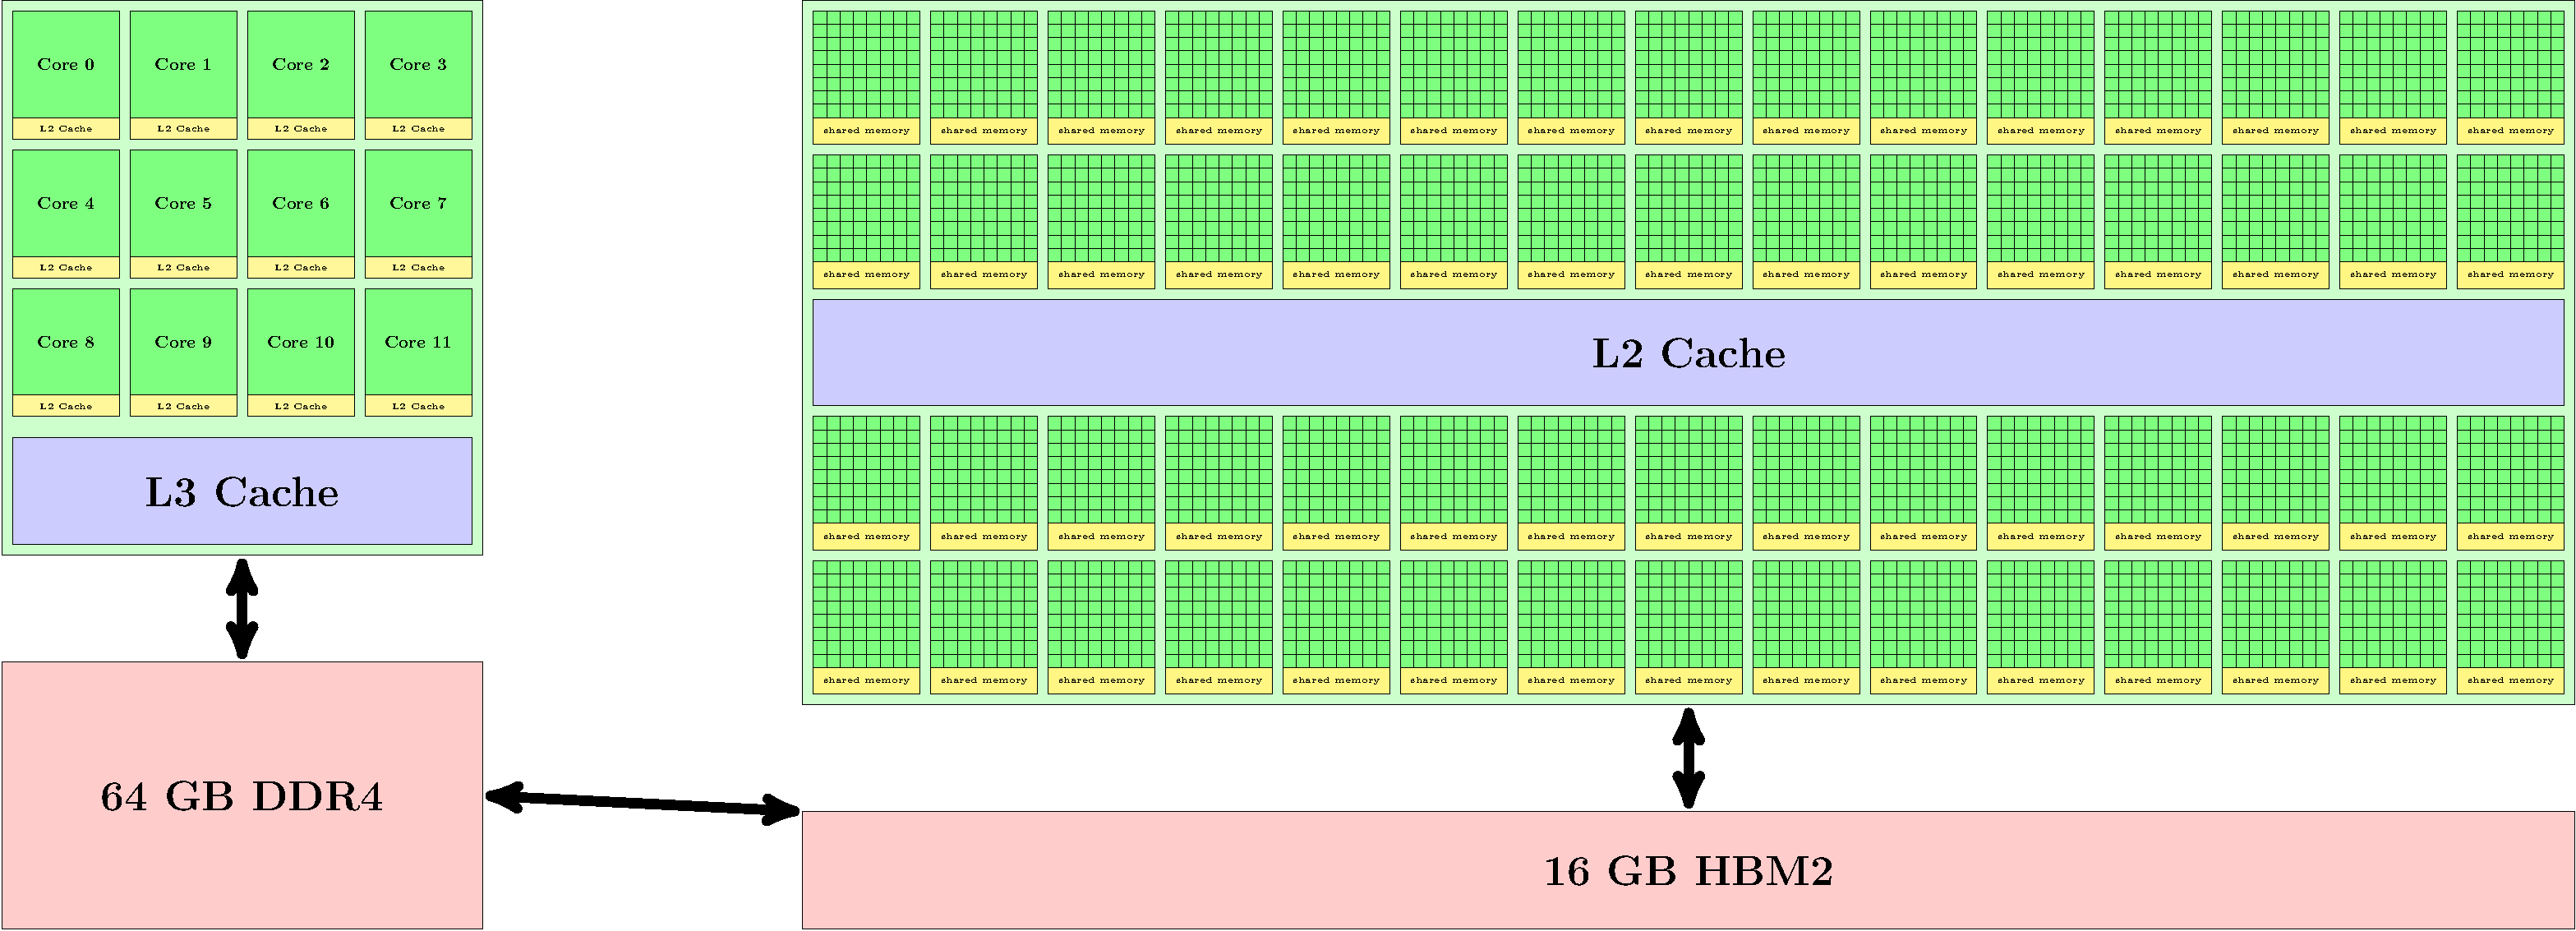
\includegraphics[width=\textwidth]{pizdaint_node}
  \end{figure}
\end{frame}

\begin{frame}{MPI and the free lunch}
  HPC applications were ported to use the message passing library MPI in the late 90s and early 2000s at great cost and effort
  \begin{itemize}
  \item Individual nodes with one or two CPUs
  \item Break problem into chunks/sub-domains
  \item Explicit message passing between sub-domains
  \end{itemize}

  The free lunch was the regular speedup in codes as CPU clock frequencies increased and as the number of nodes in systems increased
  \begin{itemize}
  \item With little/no effort, each new generation of processor bought significant speedups
  \end{itemize}
  \dots but there is no such thing as a free lunch
\end{frame}

\begin{frame}{The Moore's Law}
  \begin{figure}
    \centering
    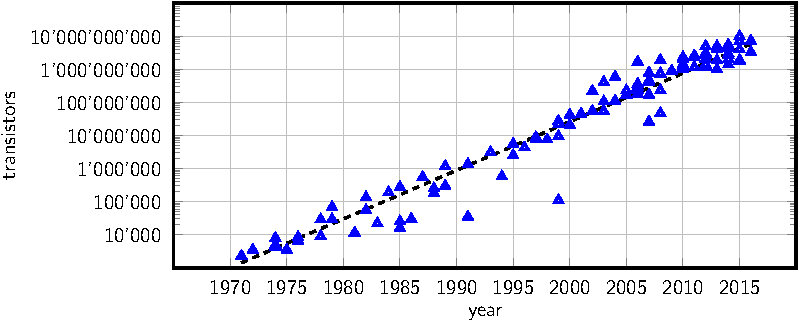
\includegraphics[width=.8\textwidth]{transistors_growth}
  \end{figure}
  \small
  \vspace{-.5\baselineskip}\centering
  \emph{Transistor density doubles every 18 months.}
\end{frame}

\begin{frame}{The Power Wall}
  \begin{figure}
    \centering
    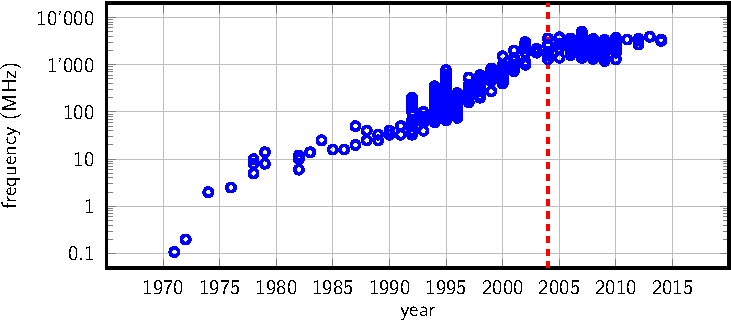
\includegraphics[width=.8\textwidth]{freq_scaling}
  \end{figure}
  \vspace{-.5\baselineskip}\centering
  $\mathbf{power} \propto \mathbf{frequency}^3$
\end{frame}

\begin{frame}{The Power Wall}
  \begin{figure}
    \centering
    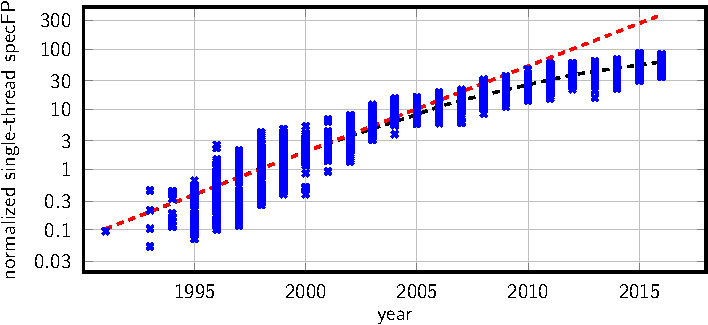
\includegraphics[width=.8\textwidth]{fp_perf}
  \end{figure}
   \vspace{-.5\baselineskip}\centering
   \emph{Floating point performance per core is not keeping up}
\end{frame}


\begin{frame}{How to speed up an application}
  There are three ways to increase performance:
  \vfill
  \begin{enumerate}
  \item Increase clock speed
  \item Increase the number of operations per clock cycle:
    \begin{itemize}
    \item Vectorization
    \item Instruction level parallelism
    \item More cores
    \end{itemize}
  \item Don't stall
    \begin{itemize}
    \item e.g., increase cache reuse to avoid waiting on memory requests
    \item e.g., branch prediction to avoid pipeline stalls
    \end{itemize}
  \end{enumerate}
\end{frame}

\begin{frame}{Clock frequency won't increase}
  In fact, clock frequencies have been going down as the number of cores increases
  \begin{itemize}
  \item A 4-core Haswell processor at 3.5\,GHz (4$\times$3.5$=$14\,Gops/s) has the same power consumption as a 12-core Haswell at 2.6\,GHz (12$\times$2.6$=$31\,Gops/s)
  \item A P100 GPU with 3582 CUDA cores runs at 1.1\,GHz
  \end{itemize}
  \vfill
  \emph{It is not reasonable to compare directly a CUDA core and an X86 core.}
\end{frame}

\begin{frame}{Parallelism will increase}
  \begin{itemize}
  \item The number of cores in both CPUs and accelerators will continue to increase
  \item The width of vector lanes in CPUs will increase
    \begin{itemize}
    \item Currently 4 doubles for AVX2
    \item Increase to 8 double for AVX512 (KNL and Skylake)
    \end{itemize}
  \item The number of threads per core will increase
    \begin{itemize}
    \item Intel Haswell: 2\,threads/core
    \item Intel KNL: 4\,threads/core
    \item IBM Power8: 8\,threads/core
    \end{itemize}
  \end{itemize}
\end{frame}

\begin{frame}{Low latency or high throughput}
  \begin{minipage}{.7\textwidth}
    CPU
    \begin{itemize}
    \item Optimized for low-latency access to cached data sets
    \item Control logic for out-of-order and speculative execution
    \end{itemize}
    GPU
    \begin{itemize}
    \item Optimized for data-parallel, throughput computation
    \item Architecture tolerant of memory latency
    \item More transistors dedicated to computation
    \end{itemize}
  \end{minipage}
  \begin{minipage}{.29\textwidth}
    \begin{figure}
      \centering
      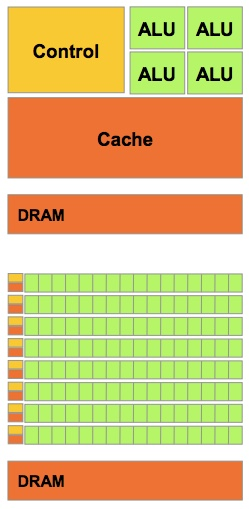
\includegraphics[height=.75\textheight]{layout.jpg} \\
    \end{figure}
    \vspace{-\baselineskip}
    \raggedleft
    \scriptsize
    \emph{\textcopyright\ NVIDIA Corp. 2010}
  \end{minipage}
\end{frame}

\begin{frame}{GPUs are throughput devices}
  \begin{itemize}
  \item CPU cores are optimized to minimize latency between operations
  \item GPUs aim to minimize latency between operations by scheduling multiple warps (thread bundles).
  \end{itemize}
  \begin{figure}
    \centering
    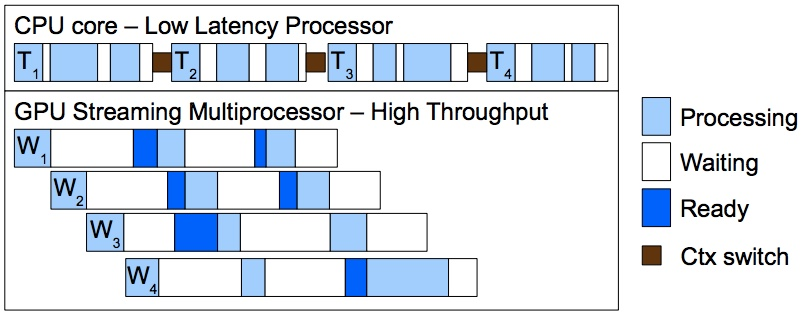
\includegraphics[width=.7\textwidth]{latency.jpg}
  \end{figure}
  \begin{flushright}
    \vspace{-\baselineskip}
    \raggedleft
    \scriptsize
    \emph{\textcopyright\ NVIDIA Corp. 2010}
  \end{flushright}
\end{frame}

\begin{frame}{Current applications not designed for many-core}
  \begin{itemize}
  \item Exposing sufficient fine-grained parallelism for multi- and many-core processors is hard
  \item New programming models are required
  \item New algorithms are required
  \item Existing code has to be rewritten or refactored
  \end{itemize}
  \pause
  \dots and compute nodes are under-utilized
  \begin{itemize}
  \item Users are not getting the most out of allocations
  \item The amount of parallelism on-node is only going to increase!
  \end{itemize}
\end{frame}


\part{Understanding the GPU architecture}

\begin{frame}{Architecture overview}{The P100 GPU (Pascal architecture)}
  \begin{figure}
    \centering
    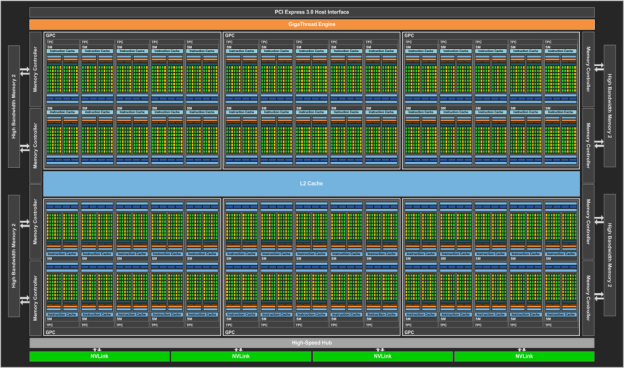
\includegraphics[scale=.9]{p100_arch.png} \\
    \emph{\scriptsize\textcopyright\ NVIDIA Corp. 2016}
  \end{figure}
\end{frame}

\begin{frame}{The SM architecture}
  \begin{minipage}{.74\textwidth}
    \small
    \begin{itemize}
    \item Multiple lightweight single-threaded cores (64 on P100)
    \item Synchronous execution on groups of 32 threads/cores
      \begin{itemize}
      \item All 32 cores execute the same instruction
      \end{itemize}
    \item Very large register file partitioned per core (256\,KB)
    \item Warp scheduler
      \begin{itemize}
      \item Picks up the next ready warp
      \item Very fast warp switching
      \end{itemize}
    \item User-managed shared fast memory (64\,KB on P100)
    \end{itemize}
  \end{minipage}
  \begin{minipage}{.25\textwidth}
    \begin{figure}
      \centering
      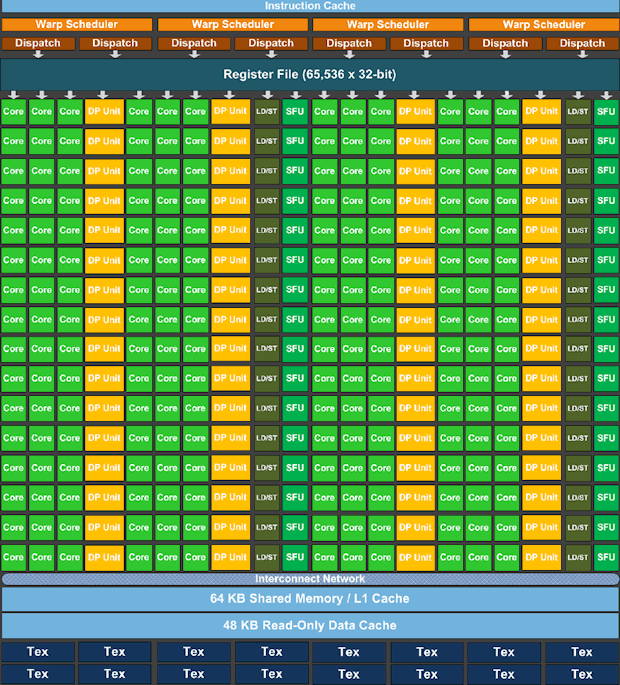
\includegraphics[width=\textwidth,height=.7\textheight]{smx_arch.png}
    \end{figure}
    \begin{center}
      \vspace{-\baselineskip}
      \emph{\scriptsize\textcopyright\ NVIDIA Corp. 2012}
    \end{center}
  \end{minipage}
\end{frame}

\begin{frame}{Execution model}
  Host-directed execution
  \begin{itemize}
  \item CPU sets up and launches \emph{kernels} on the GPU
  \item CPU manages the memory on the GPU
    \begin{itemize}
    \item Allocations, transfers in and out of the GPU
    \end{itemize}
  \end{itemize}
  \pause\vfill
  Unified memory between CPU and GPU
  \begin{itemize}
  \item Virtual address space shared between CPU and GPU
  \item The CUDA driver and the hardware take care of the page migration
  \item Introduced with Kepler, significantly improved with Pascal
  \end{itemize}
\end{frame}


\begin{frame}{Execution model}{How this huge parallelism is managed on the GPU?}
  \begin{itemize}
  \item An application launches \emph{kernels} to be executed on the GPU
  \item Each kernel comprises several \emph{blocks} of threads
  \item A thread block may only run on a single SM
  \item Multiple thread blocks might be accomodated in a single SM, if\dots
    \begin{itemize}
    \item there are enough registers,
    \item there is enough shared memory or
    \item hardware limits are not reached (active warps)
    \end{itemize}
  \item Warps of any \emph{active} block may be scheduled to run on the SM cores
  \end{itemize}
\end{frame}


\begin{frame}{Execution model}{Implications}
  \begin{itemize}
  \item Lots of parallelism is needed to cover execution latencies
    \begin{itemize}
    \item Enough warps must be available for scheduling
    \end{itemize}
    \vfill
  \item Global synchronization is not possible
    \begin{itemize}
    \item Not all the blocks of a kernel run simultaneously
    \item \emph{Synchronization is only possible within the threads of a block}
    \end{itemize}
    \vfill
  \item If program's control flow diverges within a warp $\rightarrow$ redundant execution
    \begin{itemize}
    \item Both branches are executed by the warp redundantly
    \end{itemize}
  \end{itemize}
\end{frame}


\begin{frame}{Memory model}{Memory hierarchy}
  \begin{enumerate}
  \item Global high bandwidth memory (558\,GB/s on P100)
    \begin{itemize}
    \item Accessible from all SMs
    \end{itemize}
  \item L1 cache/Shared memory
    \begin{itemize}
    \item Shared within an SM
    \item One-cycle access latency (best case)
    \item User or hardware managed
    \item No cache coherency across SMs
    \item No sequential consistency $\rightarrow$ enforced by synchronization primitives
    \end{itemize}
  \item L2 cache
    \begin{itemize}
    \item Hardware managed, shared across all SMs
    \end{itemize}
  \end{enumerate}
\end{frame}


\begin{frame}{How to program the GPUs?}
  \begin{itemize}
  \item CUDA
    \begin{itemize}
    \item C/C++ language extensions
    \item Low-level, lots of code
    \item Requires a good understanding of the GPU architecture
    \end{itemize}
    \vspace\baselineskip
  \item Using directives OpenACC/OpenMP
    \begin{itemize}
    \item Easy to use and productive
    \item High-level, non-intrusive changes in the code
    \item More on it, after lunch\dots
    \end{itemize}
  \end{itemize}
\end{frame}


% THANK YOU SLIDE
\cscsthankyou{Thank you for your attention}

\end{document}
